
\def \Subject {تحلیل احساسات روی ویدئوهای نقد فیلم‌‌های سینمایی}
\def \Course {درس پردازش زبان‌های طبیعی}
\def \Author {حوریه سبزواری}
\def \Report {گزارش فاز اول}
\def \StudentNumber {98412004}

\begin{center}
\vspace{.4cm}
{\bf {\huge \Subject}}\\
{\bf \Large \Course}
\vspace{.2cm}
\end{center}
{\bf \Author }  \\
{\bf شماره دانشجویی:\ \StudentNumber}
\hspace{\fill} 
{\Large \Report} \\
\hrule
\vspace{0.8cm}

\clearpage

%\huge{\Subject}\\[1.5 cm]
%\chapterauthor{\Author~ : \StudentNumber}
\par
موضوع پروژه تسک \texttt{sentiment analysis} روی ویدیو‌های نقد و بررسی فیلم‌های سینمایی است. داده‌ها از منتقدهای مشغول به فعالیت در پلتفرم یوتیوب جمع‌آوری می‌شود. در انتها برای هر داده‌ی ورودی مشخص می‌گردد که نظر کلی ویدیو راجع به آن فیلم سینمایی خوب، متوسط یا بد بوده است.\\ \\
لینک \lr{Repository}: \href{https://github.com/lhoorie/SentimentAnalysisOnReviewVideos}{https://github.com/lhoorie/SentimentAnalysisOnReviewVideos}

\section{منبع دقیق داده}
منبع جمع‌آوری داده فیلم‌های 2 کانال یوتیوب بنام‌های \lr{Jeremy Jahns} و \lr{Chris Stuckmann} 
بوده است. تلاش بر این بوده که داده‌ها به صورت متوازن از هر سه برچسب انتخاب و استخراج شوند.

\section{روش جمع‌آوری، مراحل و ابزارهای استفاده‌شده در جمع‌آوری داده}
 در مراحل این پروژه از کتابخانه‌های زیر برای عنوان‌های ذکرشده استفاده شده‌است:
\begin{itemize}
\item
 کتابخانۀ 
\texttt{YouTubeTranscriptApi} برای گرفتن زیرنویس ویدئوهای داخل دیتاست
\item
  کتابخانۀ 
 \texttt{YouTube} برای استخراج نام فیلم 
 \item
  کتابخانۀ 
 \texttt{extract} برای استخراج \texttt{id} از لینک ویدئو 
 \item
  کتابخانۀ \texttt{nltk} برای \texttt{tokenize} کردن جملات
 \item
  کتابخانۀ \texttt{NNSplit} برای جمله‌بندی زیرنویس‌ها
  \item
  کتابخانۀ \texttt{re} برای تمیز کردن جملات
  \item 
  کتابخانۀ \texttt{pandas} برای ساختن دیتافریم‌ها
  \item و سایر کتابخانه‌های کمکی..
 \end{itemize}

 برای جمع‌آوری داده ابتدا لینک‌های 90 فیلم از کانال‌های ذکرشده به صورت متوازن انتخاب شده است. سپس زیرنویس هر لینک استخراج شده و توابع موجود در کد روی آن اعمال می‌شوند. در انتها نیز اطلاعات مربوطه به صورت \lr{data frame} درآمده و در فایل‌های \lr{csv} ذخیره می‌شوند.

\clearpage


\section{فرمت داده‌ها}
همانطور که در پروژه ذکر شده بود، فرمت داده‌های پروژه به صورت زیر است:
\begin{itemize}
    \item پوشۀ \texttt{data} شامل دو زیرپوشه به نام‌های \texttt{rawdata} و \texttt{cleandata} است که هرکدام شامل یک فایل \texttt{csv} از دادۀ خام و دادۀ تمیز است.
    \item پوشۀ \texttt{src} شامل یک فایل \texttt{notebook} کدهای پروژه است.
    \item پوشۀ \texttt{stats} شامل فایل‌های \texttt{csv} آمارهای خواسته شده است.
\end{itemize}
برچسب‌ها به صورت سه عدد 0 و 1 و 2 هستند. برچسب 0 به معنای نظر منفی، برچسب 1 به معنای نظر خنثی و برچسب 2 به معنای نظر مثبت منتقد است.

\section{پیش‌پردازش‌های انجام شده}
\subsection{روش/ابزار تفکیک جملات}
همانطور که می‌دانیم در زیرنویس ویدئوها علائمی مانند نقطه وجود ندارد و واحد آن عباراتی است که برای چند ثانیه روی قسمتی از فیلم می‌آیند. لذا من با استفاده از ابزار \texttt{NNSplit} جملاتی حدودی به ازای هر زیرنویس استخراج کردم
\texttt{NNSplit} یک کتابخانه برای تقسیم‌بندی متن است که از شبکه‌های عصبی برای انجام تشخیص مرز جمله استفاده می کند. با آموزش یک مدل یادگیری عمیق بر روی مجموعۀ بزرگی از داده‌های متنی کار می‌کند تا مکان‌هایی را که جملات شروع و پایان می‌دهند را شناسایی کند.

\subsection{روش/ابزار تفکیک توکن‌ها/کلمات}
توکن‌های ورودی مجموعۀ کلمات زیرنویس هر ویدئو هستند. برای بدست‌آوردن کلمات به راحتی می‌توانیم از ابزار \texttt{nltk.word-tokenize()} استفاده کنیم.

\subsection{روش/معیارهای تمیزکردن داده}
پس از مشاهدۀ چند نمونه زیرنویس متوجه شدم که زیرنویس‌ها بدون علائم نگارشی، کلمات اضافی، لینک و .. هستند و به نوعی داده‌های استخراج‌شده از ابتدا تمیز بودند. اما برای اطمینان تابعی بنام \lr{clean data} تعریف کردم که موارد زیر را حذف می‌کند:
\begin{itemize}
    \item تمام عباراتی که با \texttt{@} آغاز می‌شوند
    \item تمام علائم نگارشی موجود در متن
    \item تمام \texttt{URL} ها و ارجاعات
\end{itemize}

\clearpage

\subsection{اندازۀ داده قبل/بعد از تمیز کردن داده}
همانطور که در موارد قبلی ذکر شد، داده‌ی خام موارد زیادی برای تمیز کردن نداشت و صرفا دارای کلمات بود. حتی برای پیدا کردن تعداد جملات، بدلیل عدم وجود نقطه و علائم نگارشی از کتابخانه‌های \lr{sentence detection} استفاده شد. لذا اندازه‌ی داده قبل/بعد از اعمال عملیات تمیزکردن تغییری نداشته است.

\section{واحد و روش برچسب‌گذاری}
واحد برچسب‌گذاری به صورت هر ویدئو و در واقع هر زیرنویس بوده است. همچنین برای روش برچسب‌گذاری ابتدا قصد داشتم تا تسک \lr{sentiment analysis} را بر روی نظرات هر ویدئو اعمال کنم اما پس از بررسی متوجه شدم که نظرات هر ویدئو متفاوت با برچسب خود ویدئو است. برخی راجع به خود فیلم و برخی راجع به ویدئوی نقد نظر داده بودند. لذا استفاده از این روش دارای خطای بسیاری بود. سپس تلاش کردم که از روی \texttt{imdb} هر فیلم برچسب آن را تعیین کنم که باز هم دارای خطا بود. زیرا برخی از ویدئوهای نقد صرفا با امتیاز آن فیلم همخوانی نداشت. در انتها مجبور به برچسب‌گذاری دستی شدم که دارای خطای کمینه و دقت بیشینه بود. بدین منظور از سایت \texttt{www.rottentomatoes.com} نیز کمک گرفته شد.

\section{آمار داده}
\subsection{تعداد واحد داده}
\begin{center}
\csvautotabular{stats/df_a.csv}
\end{center}
\subsection{تعداد جملات}
\begin{center}
\csvautotabular{stats/df_b.csv}
\end{center}
\subsection{تعداد کلمات}
\begin{center}
\csvautotabular{stats/df_c.csv}
\end{center}

\clearpage

\subsection{تعداد کلمات منحصربه‌فرد}
\begin{center}
\csvautotabular{stats/df_d.csv}
\end{center}

\subsection{تعداد کلمات منحصربه‌فرد مشترک و غیرمشترک بین برچسب‌ها}
\begin{center}
\csvautotabular{stats/df_e.csv}
\end{center}

\subsection{10 کلمه پرتکرار غیرمشترک هر برچسب }
\begin{center}
\csvautotabular{stats/df_f.csv}
\end{center}

\subsection{10 کلمه برتر هر برچسب بر اساس معیار  \texttt{Relative-Normalized-Frequency}}
\begin{center}
\csvautotabular{stats/df_g.csv}
\end{center}

\clearpage

\subsection{10 کلمه برتر هر برچسب بر اساس معیار \texttt{TF-IDF}}
\begin{center}
\csvautotabular{stats/df_h.csv}
\end{center}

\subsection{هیستوگرام تعداد تکرار هر کلمه منحصربه‌فرد به ترتیب از فرکانس بالا به پایین}
\begin{figure}[htbp]
  \centering
  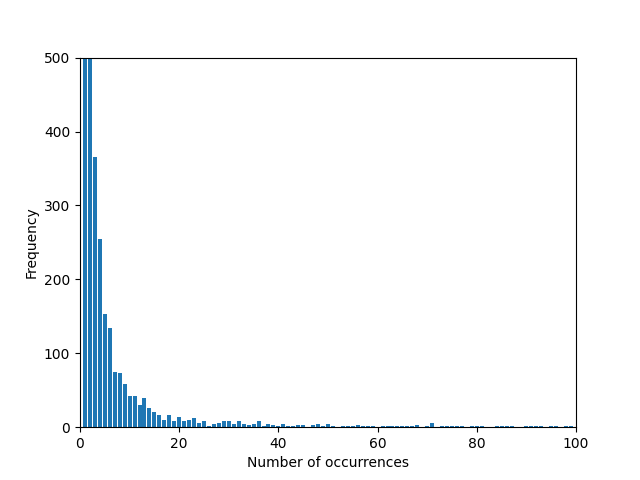
\includegraphics[width=0.7\textwidth]{stats/histogram_0.png}
  \caption{برچسب 0}
  \label{fig:example}
\end{figure}

\begin{figure}[htbp]
  \centering
  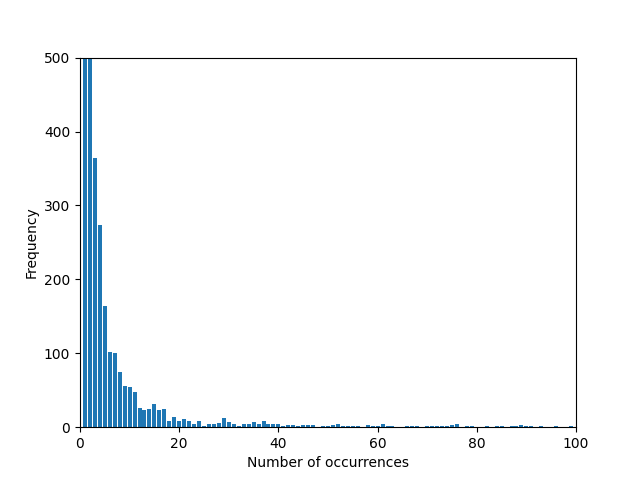
\includegraphics[width=0.7\textwidth]{stats/histogram_1.png}
  \caption{برچسب 1}
  \label{fig:example}
\end{figure}

\begin{figure}[htbp]
  \centering
  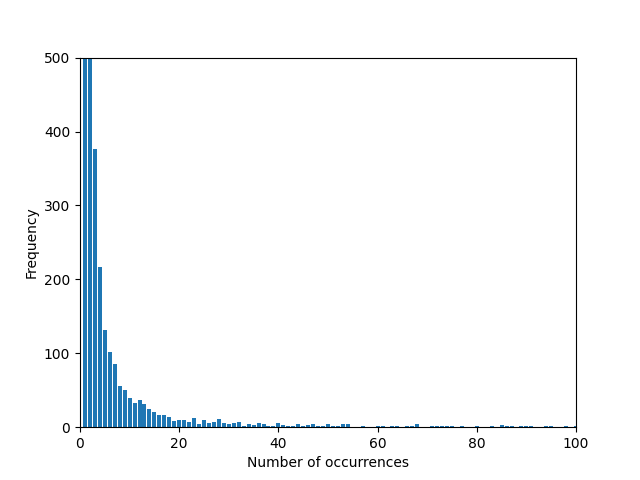
\includegraphics[width=0.7\textwidth]{stats/histogram_2.png}
  \caption{برچسب 2}
  \label{fig:example}
\end{figure}